\section{Transformation: Pattern Variable Resolution}

\subsection{Algorithm}

Immediately after parsing Redex specification, it is unknown whether certain elements of pattern are built-in patterns or non-terminal symbols or just literals. These elements will be represented with \UnresolvedSymbol instances. Given $DefineLanguage df$, let $Nts(df)$ be the set of all non-terminal symbols of the language. By analyzing $s$ in \UnresolvedSymbol using $Nts(df)$ and buildin pattern names (TODO) it is possible to termine if given \UnresolvedSymbol is either \Nt, \BuiltInPattern, or \LiteralPattern.

The symbol is analyzed in the following way: locate first underscore character. If there are no underscore characters, simply return the symbol, otherwise return all characters before the underscore. If underscore is the first character of the symbol, raise an `Exception` because Redex doesn't consider such symbols valid. Resulting symbol will be refered to as \textit{prefix}.

This transformation is applicable to all patterns as well as \texttt{define-language} form. In case of \texttt{define-language}, need to maintain variables used in patterns in order to make \texttt{variables-not-otherwise-mentioned} pattern work. Let $V = \{\}$ be the set of all variables defined in the language. 

Resolution algorithm proceeds in the following manner. The pattern is traversed recurisely. When coming across \UnresolvedSymbol node, extract prefix from the symbol $s$.  


\begin{itemize}
\item
Prefix is \texttt{number}, replace \UnresolvedSymbol with  \BuiltInPattern with $t=Number$ and $s$ defined above.

\item
Prefix is \texttt{integer}, replace \UnresolvedSymbol with  \BuiltInPattern with $t=Integer$ and $s$ defined above.

\item
Prefix is \texttt{real}, replace \UnresolvedSymbol with  \BuiltInPattern with $t=Real$ and $s$ defined above.

\item
Prefix is \texttt{natural}, replace \UnresolvedSymbol with  \BuiltInPattern with $t=Natural$ and $s$ defined above.

\item
Prefix is \texttt{string}, replace \UnresolvedSymbol with  \BuiltInPattern with $t=String$ and $s$ defined above.

\item
Prefix is \texttt{boolean}, replace \UnresolvedSymbol with  \BuiltInPattern with $t=Boolean$ and $s$ defined above.

\item
Prefix is \texttt{variable-not-otherwise-mentioned}, replace \UnresolvedSymbol with  \BuiltInPattern with $t=Variable$ and $s$ defined above.

\item
* Prefix is \texttt{hole}, replace \UnresolvedSymbol with  \BuiltInPattern with $t=Variable$ and $s$ defined above. PltRedex does not allow underscores for \texttt{hole} patterns and thus raise Exception if prefix $\neq s$.

\item
Prefix $p$ is found in the list of non-terminal symbols defined by the language, replace unresolved symbol with \Nt with $nt=p$ and $s$ defined above.

\item
Finally, check that symbol contains no underscores. Redex only allows underscores after non-terminal symbols and built-in patterns. Abort compilation if that is the case. Otherwise, replace unresolved symbol with \LiteralPattern with $l=Variable$, $v=s$ and $V = V \cup \{s\}$.

\end{itemize}

If transformation was performed on \texttt{define-language}, annotate $DefineLanguage$ with $V$.


\subsection{Example}

\begin{figure}[H]
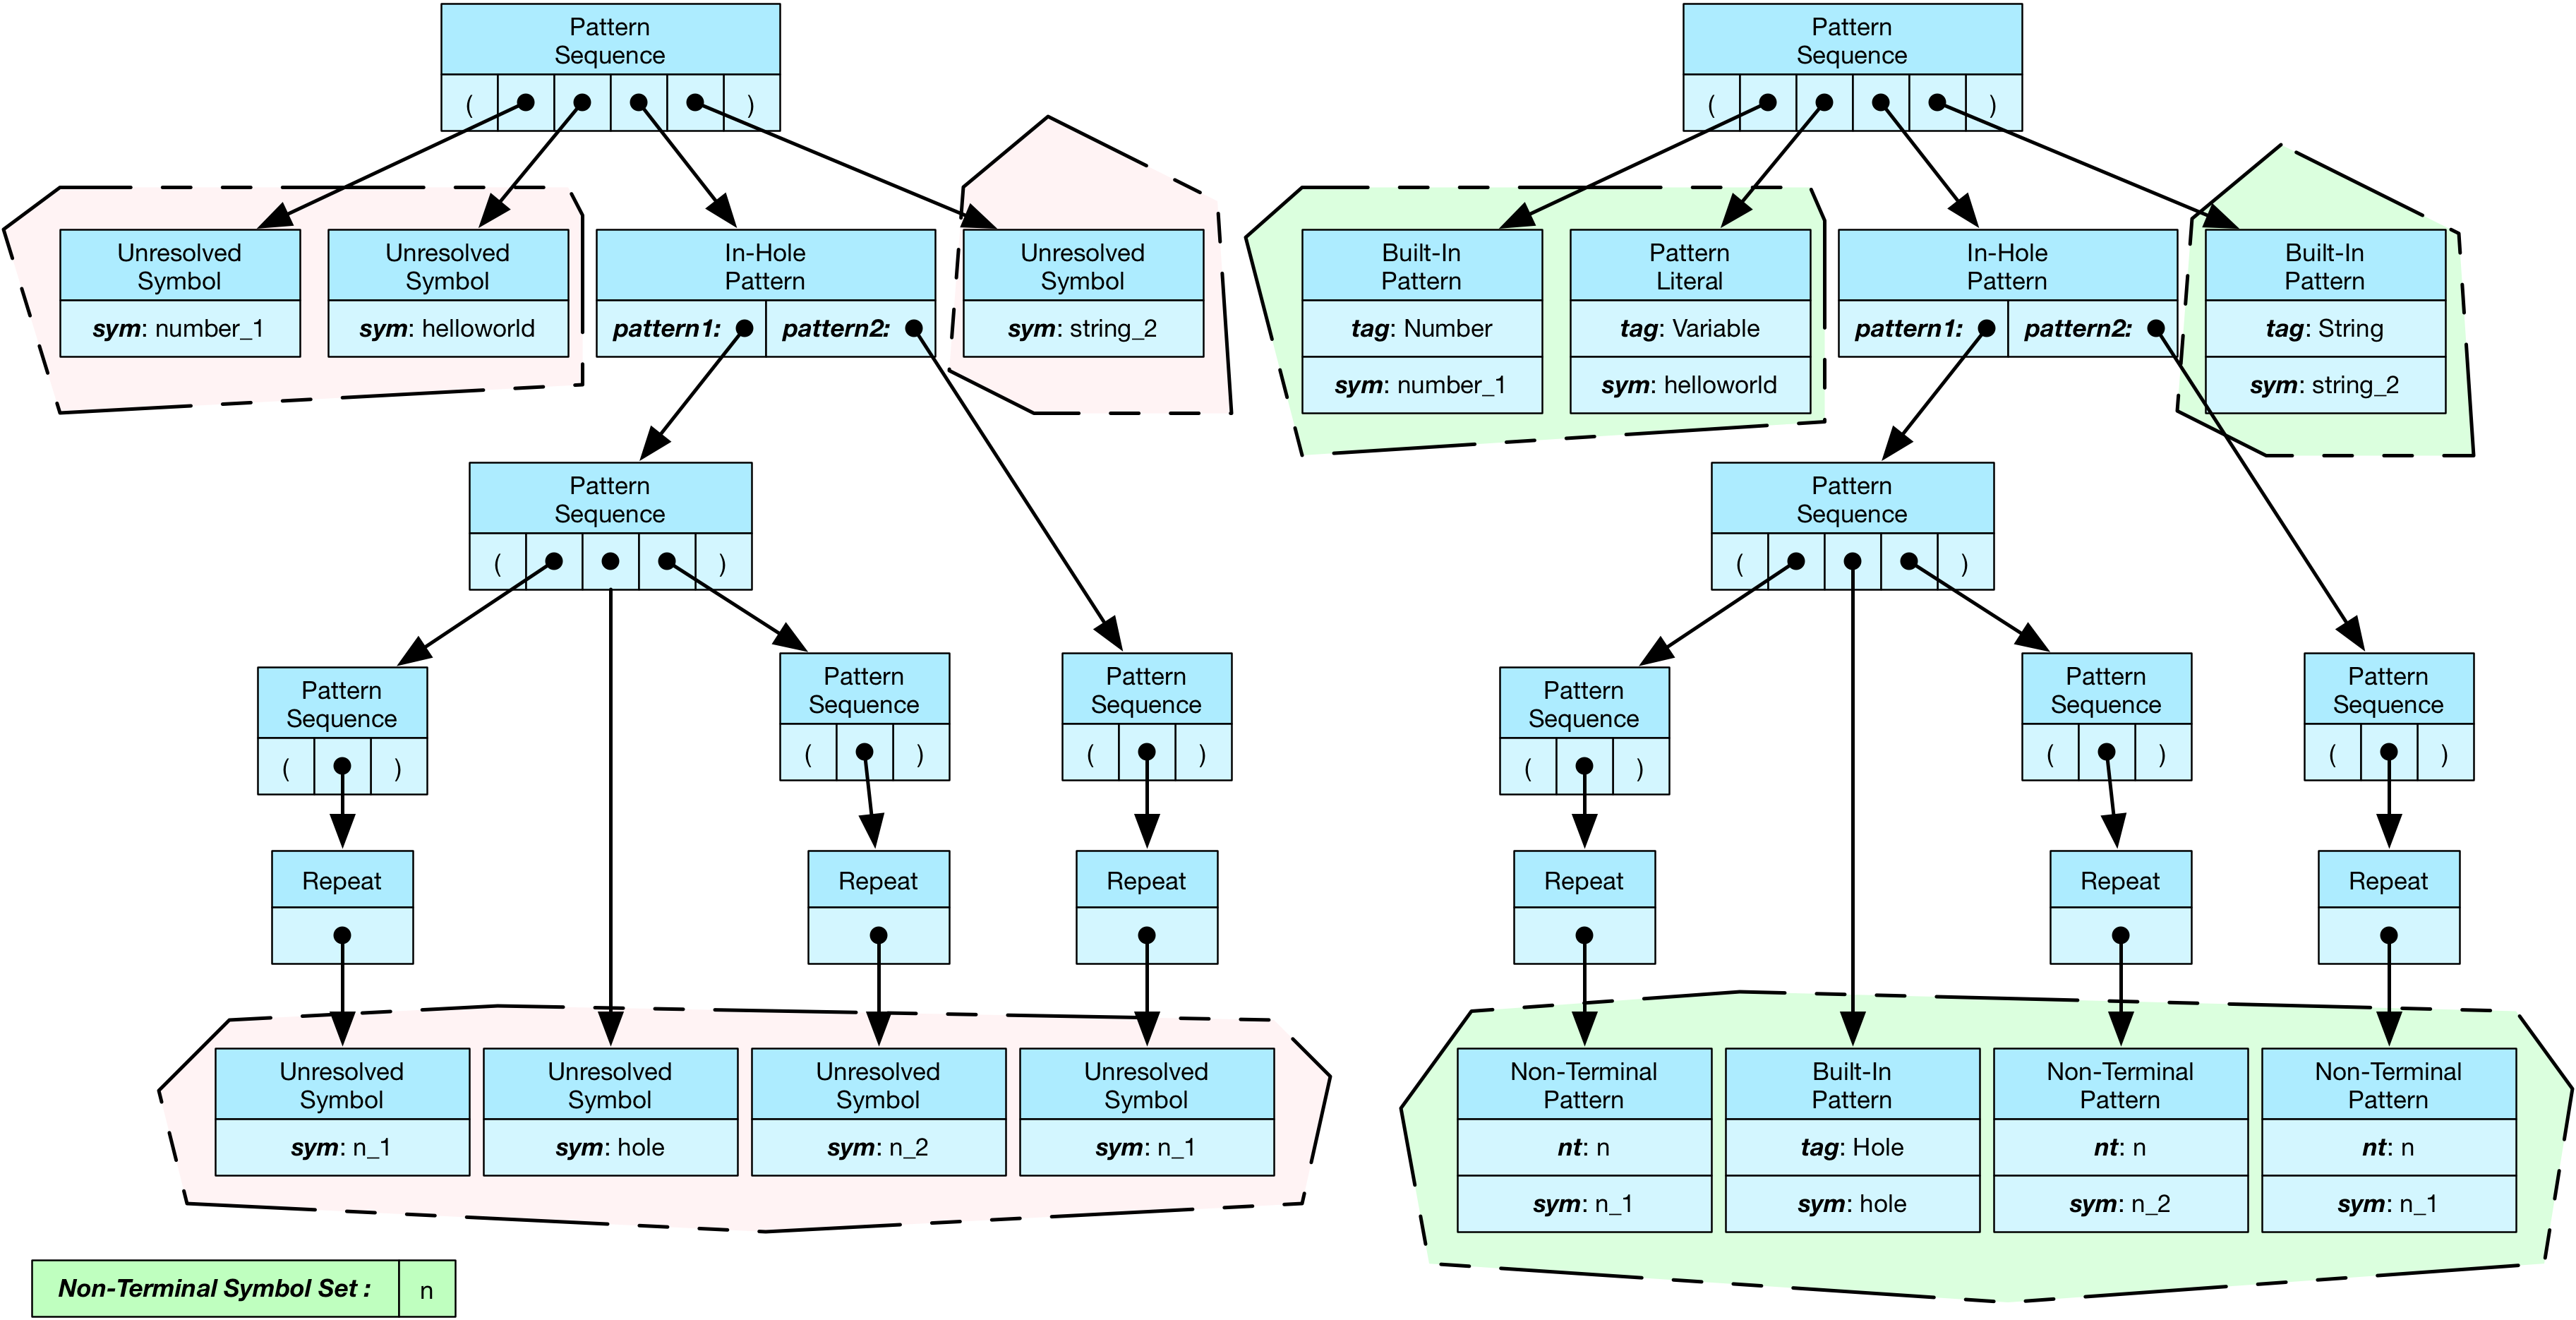
\includegraphics[scale=0.11]{transformation-pattern-resolvesym.png}
\caption{Pattern before and after pattern variable resolution.}
\label{transformation-pattern-resolvesym}
\end{figure}

Figure \ref{transformation-pattern-resolvesym} shows an effect of transformation on pattern \texttt{(number\_1 helloworld (in-hole ((n\_1 ...) hole (n\_2 ...)) (n\_1 ...)) string\_2)}. Assume related \texttt{define-language} has a single non-terminal \texttt{n}. Initially the pattern has six unresolved symbols - \texttt{number\_1}, \texttt{helloworld}, \texttt{n\_1}, \texttt{n\_2}, \texttt{hole} and \texttt{string\_2}. \texttt{number\_1}, \texttt{string\_2} and \texttt{hole} become \texttt{BuiltInPattern} with appropriate tags,  \texttt{n\_1} and \texttt{n\_2} turn into non-terminals because prefix \texttt{n} is in the set of non-terminal symbols of given \texttt{define-language} and \texttt{helloworld} becomes a \texttt{LiteralPattern} with tag \texttt{Variable}. If this pattern were a part of \texttt{define-language}, \texttt{helloworld} would have been included into set $V$.
